\documentclass[12pt,letter]{article}
\usepackage[moduleName={Mega Tone}]{KautenjaDSP}
% import a debugging package to show the margin boxes
% \usepackage{showframe}
% set the graphics path to the img directory
\graphicspath{{img/}}

% algorithm2e stuff
% \SetKwInOut{Objects}{$\CKmatrix{O}$}
% \SetKwInOut{Weights}{$\CKvector{w}$}

\begin{document}
\titlePage{Logo}{Module}{KautenjaDSP}

% -------------------
% MARK: Overview
% -------------------

\section*{Overview}

Mega Tone is an emulation of the Texas Instruments SN76489 audio processing unit from the Sega Master System, Sega Mega Drive, and Sega Genesis. The SN76489 chip contains three pulse waveform generators and an LFSR-based noise generator that selects between pitched white-noise and static periodic noise. Mega Tone provides the key features of the SN76489 chip, namely,
\begin{itemize}
  \item \textbf{Triple Pulse Waveform Generator:} Three 8-bit pulse waves with $50\%$ duty cycle and 10-bit frequency parameter
  \item \textbf{Noise Generator:} Generate either pitched white-noise based on the frequency of oscillator three, or static periodic noise at one of three shift frequencies: $\frac{N}{2048}$, $\frac{N}{1024}$, $\frac{N}{512}$ where $N$ is the reference clock rate (which is something like $3579545Hz$).
  \item \textbf{4-bit Amplifier:} A 4-bit amplifier controls the output level of each oscillator with mixer sliders and CV inputs
  \item \textbf{Channel Mixer:} Mix the voices together internally with hard clipping and aliasing.
\end{itemize}

% -------------------
% MARK: Panel Layout
% -------------------

\clearpage
\section*{Panel Layout}

\begin{figure}[!htp]
\centering
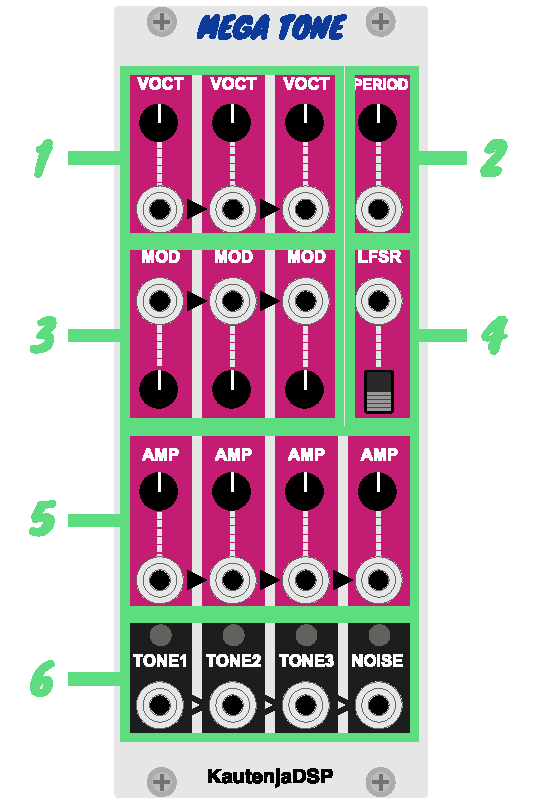
\includegraphics[width=0.4\textwidth]{Interface}
\end{figure}

\subsection*{1{\quad}Tone Generator Frequency}

The trimpot controls the coarse frequency of the three tone generators. Frequency is quantized to a 10-bit value for the oscillators, which is particularly noticeable in the very low / high registers. The ports provide an exponential $V$/Octave input for controlling the pitch of the tone generators. Inputs are normalled forward from Tone 1, to Tone 2, to Tone 3.

\subsection*{2{\quad}Noise Frequency}

The noise generator can be set to one of four settings. The first setting produces pitched white noise based on the frequency of tone generator 3. The remaining three settings produce a static pitched white noised at rates of $\frac{N}{2048}$, $\frac{N}{1024}$, $\frac{N}{512}$ where $N$ is the reference clock rate, which is something like $3579545Hz$ on the Sega consoles. The input port provides voltage control over the noise frequency setting where each discrete setting is allocated $2.5$ Volts of input range.

\clearpage
\subsection*{3{\quad}Tone Generator Frequency Modulation}

When nothing is patched to the frequency modulation port, the trimpot can be used to fine tune the frequency of the given tone generator. When a signal is patched, the input port provides linear frequency modulation to the corresponding tone generator and the trimpot can be used as an attenuverter to attenuate / polarize the incoming signal. Inputs are normalled forward from Tone 1, to Tone 2, to Tone 3.

\subsection*{4{\quad}LFSR}

When the switch is pointing up, the noise generator produces periodic noise. When pointing down, pitched white noise is generated. The input port acts like a gate that goes high at $2V$ and inverts the value of the LFSR switch.

\subsection*{5{\quad}Amplifier}

When no input is connected, the trimpot controls the level from $0\%$ to $100\%$ with 4-bit resolution. When an input is patched to the port, the trimpot acts like an attenuator that scales the CV control over the volume level. Because the amplifier has 4-bit control, the envelope of the voice will sound quantized when used with an external envelope generator. Inputs are normalled forward from Tone 1, to Tone 2, to Tone 3, to Noise.

\subsection*{6{\quad}Outputs}

Each voice produces an output signal of at most ${\approx}10V_{pp}$ when the amplifier is maxed out. The individual oscillators cannot be overdriven to produce clipping, distortion, or aliasing. However, outputs are normalled forward into a sum mix where hard clipping \textit{can} occur. Excess clipping will introduce an aliasing effect to the mix. Outputs in the mix are clipped \textit{before} being normalled to the next output. VU meter lights measure the output of individual channels going from off ($-\infty dB$ to $0dB$), to green ($-12dB$ to $0dB$), and lastly to red ($0dB$ to $3dB$) when clipping begins to occur.

% -------------------
% MARK: Data Sheet
% -------------------

\clearpage
\section*{Data Sheet}

\begin{table}[!htp]
\begin{tabular}{|l|l|}
\hline
Type             & Oscillator / Noise Generator  \\
\hline
Size             & 10 HP Eurorack           \\
\hline
Depth            & NA                       \\
\hline
Power            & NA                       \\ % 2 x 5 Eurorack
\hline
$+12V$ draw (mA) & 0 mA                     \\
\hline
$-12V$ draw (mA) & 0 mA                     \\
\hline
$+5V$ draw (mA)  & 0 mA                     \\
\hline
\end{tabular}
\end{table}

% -------------------
% MARK: References
% -------------------

\clearpage
\renewcommand\refname{References \& Acknowledgments}
\nocite{*}
\bibliographystyle{apalike}
\bibliography{references}

\end{document}
